\documentclass[twoside,11pt,openright]{report}

\usepackage[latin1]{inputenc}
\usepackage[american]{babel}
\usepackage{a4}
\usepackage{latexsym}
\usepackage{amssymb}
\usepackage{amsmath}
\usepackage{epsfig}
\usepackage[T1]{fontenc}
\usepackage{mathptmx}
\usepackage{color}
\usepackage{epstopdf}
\usepackage{microtype}
\usepackage{hyperref}
\usepackage[useregional]{datetime2}
\DTMlangsetup[en-US]{showdayofmonth=false}
\usepackage{lipsum}
\usepackage{iris}
\usepackage{heaplang}
\usepackage{tikz}
\usetikzlibrary{calc,shapes.multipart,chains,arrows}


\renewcommand*\sfdefault{lmss}
\renewcommand*\ttdefault{txtt}

\newcommand{\todo}[1]{{\color[rgb]{.5,0,0}\textbf{$\blacktriangleright$#1$\blacktriangleleft$}}}

\begin{document}

%%%%%%%%%%%%%%%%%%%%%%%%%%%%%%%%%%%%%%%%%%%%%%%%%%%%%%%%%%%%%%%%%%%%%%%

\pagestyle{empty} 
\pagenumbering{roman} 
\vspace*{\fill}\noindent{\rule{\linewidth}{1mm}\\[4ex]
{\Huge\sf TITLE HERE}\\[2ex]
{\huge\sf Mathias Pedersen, 201808137}\\[2ex]
\noindent\rule{\linewidth}{1mm}\\[4ex]
\noindent{\Large\sf Master's Thesis, Computer Science\\[1ex] 
\today \\[1ex] Advisor: Amin Timany\\[15ex]}\\[\fill]}
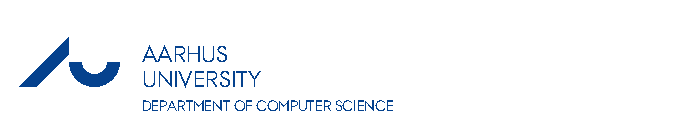
\epsfig{file=logo.eps}\clearpage

%%%%%%%%%%%%%%%%%%%%%%%%%%%%%%%%%%%%%%%%%%%%%%%%%%%%%%%%%%%%%%%%%%%%%%%

\pagestyle{plain}
\chapter*{Abstract}
\addcontentsline{toc}{chapter}{Abstract}

\todo{in English\dots}

\chapter*{Resum\'e}
\addcontentsline{toc}{chapter}{Resum\'e}

\todo{in Danish\dots}

\chapter*{Acknowledgments}
\addcontentsline{toc}{chapter}{Acknowledgments}

\todo{\dots}

\vspace{2ex}
\begin{flushright}
  \emph{Mathias Pedersen}\\
  \emph{Aarhus, \today.}
\end{flushright}

\tableofcontents
\cleardoublepage
\pagenumbering{arabic}
\setcounter{secnumdepth}{2}

%%%%%%%%%%%%%%%%%%%%%%%%%%%%%%%%%%%%%%%%%%%%%%%%%%%%%%%%%%%%%%%%%%%%%%%

\chapter{Introduction}
\label{ch:intro}

\todo{motivate and explain the problem to be addressed}

\todo{example of a citation: \cite{DBLP:conf/podc/MichaelS96}}
\todo{get your bibtex entries from \url{https://dblp.org/}}

%%%%%%%%%%%%%%%%%%%%%%%%%%%%%%%%%%%%%%%%%%%%%%%%%%%%%%%%%%%%%%%%%%%%%%%

\chapter{The Great Ideas}
\label{ch:main}

The Two-Lock Michael Scott Queue

\begin{figure}[h]
  \centering
  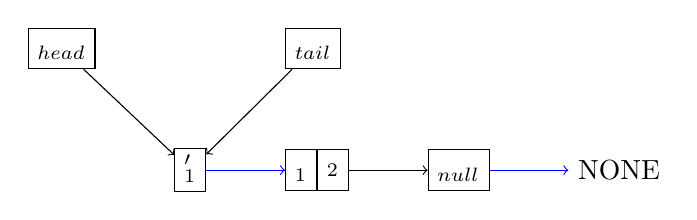
\begin{tikzpicture}[
    pair/.style = {
      on chain,
      rectangle split,
      rectangle split horizontal,
      rectangle split parts=2,
      draw,
      anchor=center,
      text height=1.5ex,
    },
    perspointer/.style = {
      on chain,
      rectangle,
      draw,
      anchor=center,
      text height=1.5ex,
    },
    pointer/.style = {
      rectangle,
      draw,
      anchor=center,
      text height=1.5ex,
    },
    start chain=going right,
  ]

  \node (l'1) [join={by ->}, perspointer,on chain] {$\loc'_1$};
  \node (l1pair) [join={by ->, draw=blue}, pair,on chain] {$\val_1$ \nodepart{two} $\loc_2$};
  \node (l'null) [join={by ->}, perspointer={a},on chain] {$\loc_{null}$};
  \node (lnull) [join={by ->, draw=blue}, rectangle,on chain] {NONE};
  \node (head) [pointer, above left=of l'1] {$\loc_{head}$};
  \node (tail) [pointer, above right=of l'1] {$\loc_{tail}$};

  \draw[->] (head) -- (l'1);
  \draw[->] (tail) -- (l'1);
  \end{tikzpicture}
  \caption{Queue after initialisation}
\end{figure}



Key insights
\begin{enumerate}
  \item\label{MSQTL:insights:head} Head always points to the first node in the queue.
  \item\label{MSQTL:insights:tail} Tail always point to either the last or second last node in the queue.
  \item\label{MSQTL:insights:persistent} All but the last pointer in the queue (the pointer to null) never change
\end{enumerate}

Insight \ref{MSQTL:insights:tail} is true, as it holds initially, and every time a new node is enqueued, the tail pointer is updated to point to the last node, and no other nodes can be enqueue before the update takes place. However, just after the new node has been linked to the queue, the tail queue will be pointing to the second last node in the queue, until it is updated in the next line.

Insight \ref{MSQTL:insights:persistent} means that we can mark all pointers in the queue (except the pointer to the null node) as persistent.

Key insights (concurrent)
\begin{enumerate}
  \item All the same as before
  \item\label{MSQTL:insights:lag} The tail can lag one node behind Head
  \item\label{MSQTL:insights:states} At any given time, the queue is in one of four states:
    \begin{enumerate}
      \item\label{MSQTL:insights:state:static} No threads are interacting with the queue (\textbf{Static})
      \item\label{MSQTL:insights:state:enqueue} A thread is enqueueing (\textbf{Enqueue})
      \item\label{MSQTL:insights:state:dequeue} A thread is dequeuing (\textbf{Dequeue})
      \item\label{MSQTL:insights:state:both} A thread is enqueueing and a thread is dequeuing (\textbf{Both})
    \end{enumerate}
\end{enumerate}

Insight \ref{MSQTL:insights:lag} might seem a little surprising, and indeed it stands in contrast to property 5 in \cite{DBLP:conf/podc/MichaelS96}, which states that the tail always points to a node in the linked list. I also didn't realise this possibility until a proof attempt using a model that "forgot" old nodes lead to an unprovable case (see section \ref{MSQTL:Discussion:xs_old}). The situation can occur when the queue is empty, and a thread performs an incomplete enqueue; it attaches the new node to the end, but before it can swing the tail node to this new node, another thread performs a dequeue, which dequeues this new node, swings the head to it. Now the tail is lagging a node behind the head.

It is not possible for the tail to point more than one node behind the head, as in order for this to happen, more nodes must be enqueued, but this can't happen before the current enqueue finishes, which will update the tail and bring it up to speed with the head.

Fortunately, this isn't an issue for safety, but a consequence of this possibility is that when modelling the queue, we must remember at least one "old" node (i.e. a dequeued node), as the tail might be pointing to this node. For the sake of simplicity in the model, the choice is made to remember an arbitrary amount of old nodes, which is represented by the list $xs_{old}$.


\subsubsection{Discussing the need for $xs_{old}$}\label{MSQTL:Discussion:xs_old}

As mentioned in the insights, it is possible for the tail to lag one node behind the head. This insight lead to including the old nodes of the queue in the queue invariant. This addition manifests in the end of the proof of dequeue. When we open the invariant to swing the head to the new node, we get that the entire queue is $xs$. After performing the write, we can then close the invariant with the same $xs$ that we opened the queue to (just written differently to signify that $x_{head}$ is now "old"). Because of this, we can supply the same predicate concerning the $tail$ (the or) that we opened the queue with, since these only mention $xs$, which remains the same.

Had we not used an $xs_{old}$ and essentially just "forgotten" old nodes in the queue, we couldn't have done this. Say that we defined $xs$ as $xs = x_{head} :: xs_{rest}$ instead. Then, once we have to close the invariant, we cannot supply the $xs$, which we got when we opened the invariant. Our only choice (due to the fact that $head$ must point to $x_{n_head}$) is to close the invariant with $xs' = xs_{rest} = x_{n_head} :: xs_{n_rest}''$. However, clearly $xs' \neq xs$, so we cannot supply the same predicate concerning the $tail$ (the or) that we got when opening the invariant, since this predicate talks about $xs$, not $xs'$. Now, if we opened the invariant in the Dequeue case, then we could assert that $last xs = last xs'$, and hence still be able close the invariant. However, if we opened the invariant in the Both case, then we would need to assert that $2last xs = 2last xs'$. This is however not provable, since it might be the case that $xs_{n_rest}''$ is empty, and hence $2last xs'$ is $None$, whereas $2last xs = x_{n_head}$.


%%%%%%%%%%%%%%%%%%%%%%%%%%%%%%%%%%%%%%%%%%%%%%%%%%%%%%%%%%%%%%%%%%%%%%%

\chapter{Conclusion}
\label{ch:conclusion}

\todo{conclude on the problem statement from the introduction}

%%%%%%%%%%%%%%%%%%%%%%%%%%%%%%%%%%%%%%%%%%%%%%%%%%%%%%%%%%%%%%%%%%%%%%%

\cleardoublepage
\addcontentsline{toc}{chapter}{Bibliography}
\bibliographystyle{plain} 
\bibliography{refs}

%%%%%%%%%%%%%%%%%%%%%%%%%%%%%%%%%%%%%%%%%%%%%%%%%%%%%%%%%%%%%%%%%%%%%%%

\cleardoublepage
\appendix
\chapter{The Technical Details}

\todo{\dots}

\end{document}

